%!TEX TS-program = xelatex
\documentclass[12pt, a4paper, oneside]{article}

\usepackage{amsmath,amsfonts,amssymb,amsthm,mathtools}  % пакеты для математики

\usepackage[english, russian]{babel} % выбор языка для документа
\usepackage[utf8]{inputenc} % задание utf8 кодировки исходного tex файла
\usepackage[X2,T2A]{fontenc}        % кодировка

\usepackage{fontspec}         % пакет для подгрузки шрифтов
\setmainfont{Linux Libertine O}   % задаёт основной шрифт документа

\usepackage{unicode-math}     % пакет для установки математического шрифта
\setmathfont[math-style=upright]{Neo Euler} % шрифт для математики

% Конкретный символ из конкретного шрифта
% \setmathfont[range=\int]{Neo Euler}

%%%%%%%%%% Работа с картинками %%%%%%%%%
\usepackage{graphicx}                  % Для вставки рисунков
\usepackage{graphics}
\graphicspath{{images/}{pictures/}}    % можно указать папки с картинками
\usepackage{wrapfig}                   % Обтекание рисунков и таблиц текстом

%%%%%%%%%%%%%%%%%%%%%%%% Графики и рисование %%%%%%%%%%%%%%%%%%%%%%%%%%%%%%%%%
\usepackage{tikz, pgfplots}  % язык для рисования графики из latex'a

%%%%%%%%%% Гиперссылки %%%%%%%%%%
\usepackage{xcolor}              % разные цвета

\usepackage{hyperref}
\hypersetup{
	unicode=true,           % позволяет использовать юникодные символы
	colorlinks=true,       	% true - цветные ссылки, false - ссылки в рамках
	urlcolor=blue,          % цвет ссылки на url
	linkcolor=black,          % внутренние ссылки
	citecolor=green,        % на библиографию
	pdfnewwindow=true,      % при щелчке в pdf на ссылку откроется новый pdf
	breaklinks              % если ссылка не умещается в одну строку, разбивать ли ее на две части?
}


\usepackage{todonotes} % для вставки в документ заметок о том, что осталось сделать
% \todo{Здесь надо коэффициенты исправить}
% \missingfigure{Здесь будет Последний день Помпеи}
% \listoftodos --- печатает все поставленные \todo'шки

\usepackage[paper=a4paper, top=20mm, bottom=15mm,left=20mm,right=15mm]{geometry}
\usepackage{indentfirst}       % установка отступа в первом абзаце главы

\usepackage{setspace}
\setlength{\parskip}{4mm}   % Расстояние между абзацами
% Разные длины в латехе https://en.wikibooks.org/wiki/LaTeX/Lengths


\usepackage{xcolor} % Enabling mixing colors and color's call by 'svgnames'

\definecolor{MyColor1}{rgb}{0.2,0.4,0.6} %mix personal color
\newcommand{\textb}{\color{Black} \usefont{OT1}{lmss}{m}{n}}
\newcommand{\blue}{\color{MyColor1} \usefont{OT1}{lmss}{m}{n}}
\newcommand{\blueb}{\color{MyColor1} \usefont{OT1}{lmss}{b}{n}}
\newcommand{\red}{\color{LightCoral} \usefont{OT1}{lmss}{m}{n}}
\newcommand{\green}{\color{Turquoise} \usefont{OT1}{lmss}{m}{n}}

\usepackage{titlesec}
\usepackage{sectsty}
%%%%%%%%%%%%%%%%%%%%%%%%
%set section/subsections HEADINGS font and color
\sectionfont{\color{MyColor1}}  % sets colour of sections
\subsectionfont{\color{MyColor1}}  % sets colour of sections

%set section enumerator to arabic number (see footnotes markings alternatives)
\renewcommand\thesection{\arabic{section}.} %define sections numbering
\renewcommand\thesubsection{\thesection\arabic{subsection}} %subsec.num.

%define new section style
\newcommand{\mysection}{
	\titleformat{\section} [runin] {\usefont{OT1}{lmss}{b}{n}\color{MyColor1}} 
	{\thesection} {3pt} {} } 


%	CAPTIONS
\usepackage{caption}
\usepackage{subcaption}
%%%%%%%%%%%%%%%%%%%%%%%%
\captionsetup[figure]{labelfont={color=Turquoise}}

\pagestyle{empty}

%%%%%%%%%% Свои команды %%%%%%%%%%
\usepackage{etoolbox}    % логические операторы для своих макросов

% Все свои команды лучше всего определять не по ходу текста, как это сделано в этом документе, а в преамбуле!

% Одно из применений - уничтожение какого-то куска текста!
\newbool{answers}
\booltrue{answers}
%\boolfalse{answers}

\usepackage{enumitem}
% бульпоинты в списках
\definecolor{myblue}{rgb}{0, 0.45, 0.70}
\newcommand*{\MyPoint}{\tikz \draw [baseline, fill=myblue,draw=blue] circle (2.5pt);}
\renewcommand{\labelitemi}{\MyPoint}

% расстояние в списках
\setlist[itemize]{parsep=0.4em,itemsep=0em,topsep=0ex}
\setlist[enumerate]{parsep=0.4em,itemsep=0em,topsep=0ex}


\title{Ценовая сегментация брендов}
\author{Большое домашнее задание по курсу <<Введение в анализ данных>> № 1}
\date{27 апреля 2019 г.}

\begin{document}

\maketitle

\tableofcontents

\section{Общая постановка задания}

Полка воды в супермаркетах довольно часто вызывает удивление. Бутылка $0.5$~л негазированной воды может стоить от $15$ рублей до $250$ рублей. Понятно, что большая часть цены имеет маленькое отношение к составу и качеству воды, скорее, цена связана с  другими аспектами, например, позиционированием бренда или логистическими издержками.

В этом задании вам предстоит присвоить брендам одной продуктовой категории один из $4$-х ценовых сегментов:

\begin{itemize}
\item  Low priced
\item  Middle priced
\item  Upper middle priced
\item  High priced
\end{itemize} 

Для того чтобы выполнить это задание, вам нужно:

\begin{enumerate} 
	\item  разбиться в команды по 2-3 человека;
	\item  выбрать продуктовую категорию;
	\item  собрать данные;
	\item  продумать методологию сегментации;
	\item  присвоить брендам ценовой сегмент.
\end{enumerate}

На выходе должна получиться таблица:

\begin{center}
\begin{tabular}{|c|c|}
	\hline 
	Бренд & Ценовой сегмент \\ 
	\hline 
	&  \\ 
	\hline 
\end{tabular} 
\end{center} 

Выбор продуктовой категории за вами.  Подбор брендов и данных - одна из ваших задач,  т.к. сбор данных - один из ключевых навыков аналитиков.  Детальнее обо всем в следующих секциях.


\section{Продуктовые категории}

Под продуктовой категорией понимаем тип продуктов\footnote{\url{https://studfiles.net/preview/3560003/}} (по иерархии из товарного маркетинга): чай, кофе, йогурт, хлеб и т.п.

 \textbf{Требования:} выбрать категорию, в которой не менее 5 брендов и не менее 15 товаров. 

\section{Сбор данных}

Данные собираются самостоятельно и вручную. Команды должны посетить $3$ магазина сети X5 Retail Group (Перекресток, Пятерочка, Карусель) и собрать информацию о товарах выбранной категории: наименование, бренд, цена, вес. 

 \textbf{Совет:} пойти в один Перекресток и в две Пятерочки.

Результат сбора данных нужно представить в виде таблицы (на каждой странице --- данные из каждого магазина), где на первой строке в левой ячейке указывается наименование супермаркета, а в соседней --- адрес.  На второй строчке --- название колонок, и начиная с третьей --- сами данные.


\begin{center}
	\begin{tabular}{|c|c|c|c|}
		\hline 
		Перекрёсток & г. Москва, ул. Дубравная, д. 34/29 &  &  \\ 
		\hline 
		Наименование & Бренд & Цена & Вес \\ 
		\hline 
		GREENF.Чай ГОЛДЕН ЦЕЙЛОН чер.лист.200г & 
		GREENFIELD
		& 
		$139.90$
		& $0.200$ \\ 
		\hline 
	\end{tabular} 
\end{center}



\section{Методология сегментации}	

Это творческий этап - именно вы должны определить ценовые границы каждого из сегментов. 

\textbf{Совет:} переведите все цены на фиксированную единицу веса.  Например, выше цена 200-граммового чая --- $139.90$ рублей, тогда цена $100$~ г этого чая: $69.95$.

Если у вас есть две позиции одного бренда, то найдите среднюю цену на бренд. Красиво получится операция группировкой с суммированием, а затем делением одного столбца на другой (БЕЗ ЦИКЛОВ!)

Как можно выстроить методологию:

\begin{enumerate}
	\item Можно ориентироваться на процентили. Выберите $3$ уровня процентилей, так что  $k_1 < k_2 < k_3$, тогда low-priced бренды --- те, цена которых от $0$ рублей $до k_1$.
	
	\item Можно посчитать среднюю цену продуктов по категории и посчитать отношение цены бренда к средней цене (будем называть отношение ---индексом), и дробить продукты на $4$ группы по такому индексу.
	
	\item Любые другие варианты, которые придумаете.
\end{enumerate}

Эту часть надо подробно расписать внутри питоновского ноутбука. Распишите максимально подробно, чтобы мы всё поняли. Прям как для тупых пишите. 

\section{Присваивание сегмента брендам}	

Когда вы переведете цены по всей категории продуктов в цены на конкретную единицу товара, остается пройтись по колонке цены и в соответствии с ней присвоить бренду один из 4 сегментов. 

Здесь вам пригодится функция numpy.select: \url{https://docs.scipy.org/doc/numpy/reference/generated/numpy.select.html}


\section{Инструменты и темы курса}		

Содержательное нутро связано с описательными статистиками. Работаем в Jupyter Notebook.

\section{Организационные вопросы}		

\subsection*{Команды}

Задание  выполняется в командах по 2-3 человека. Индивидуальные работы не будут засчитаны.

\subsection*{Дедлайн}

\begin{itemize}
\item Задание выдаем 27.04.2019
\item Задание сдаем 12.05.2019 в 23.30 на \url{anytask.org}
\end{itemize} 

\subsection*{В каком виде сдаём?} 

\begin{enumerate}
	\item  Ждем вашу собранную эксельку с данными
	\item  Ждём ipynb, в котором: 
	\begin{enumerate}
		\item Указаны все члены команды и номер группы.
		\item Прописан весь код, который читает эксельку с собранными данными и выдает эксельку с таблицей Бренд --- Ценовой сегмент.
		\item Помимо того, что вы пишете код, вы еще в текстовых ячейках оставляете комментарии - что делали, зачем, что интересно увидели. \url{https://www.youtube.com/watch?v=LLFOZ2vN7ss} 
		
		Постарайтесь делать осмысленные выводы! Не будьте мудрыми, как король: 
		
		\begin{center}
			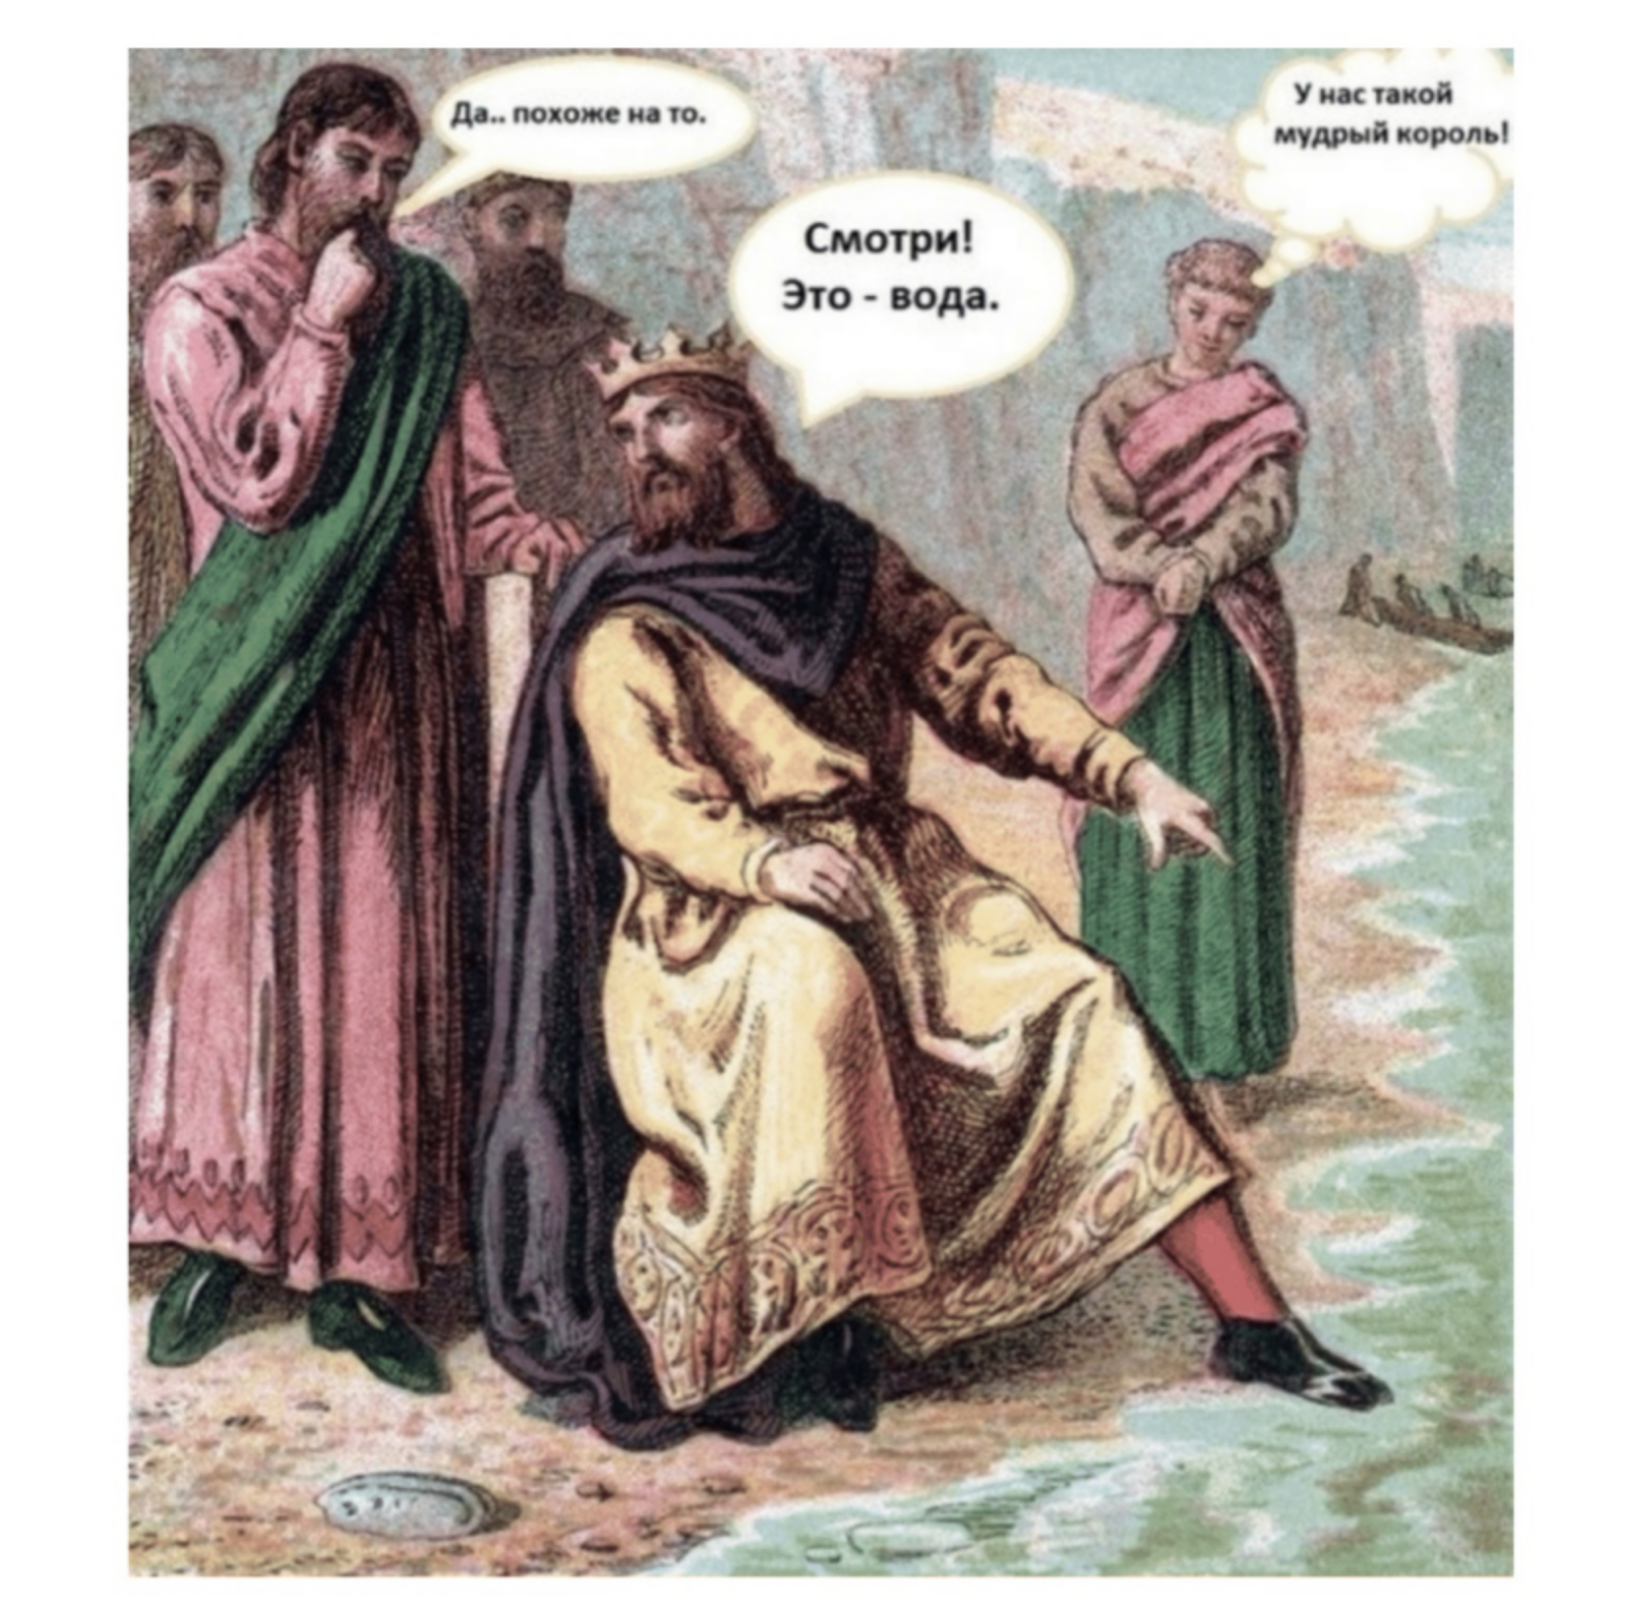
\includegraphics[scale=0.2]{laba_1.png}
		\end{center}
		
		\item Не забывайте о красивых моментах, выводите info(), head() по входному и выходному датафрейму. Красивые закономерности, найденные в данных, изображайте на картинках. 
	\end{enumerate}
\end{enumerate}

\subsection*{Оценивание}

Работа оценивается по $10$-бальной шкале.  Она ставится на команду и нормируется на число человек в ней. Так, если в команде три человека и она получает оценку $8$, она превращается в $24$ балла. Далее участники команды делят эти баллы между собой в любой пропорции в зависимости от вклада каждого участника в итоговую работу. Если в команде два участника, то $8$ соотвественно превращается в $16$.  В работе оцениваются адекватность собранных данных, чистота кода, адекватность и продуманность методологии разбиения на сегменты. 

\end{document}
